\chapter{Ламинаризации развитого турбулентного течения в трубах}\label{ch:ch3}
%

\section{Постановка задачи}\label{ch3:problem}

%
\begin{figure}[ht]
    \centerfloat{
        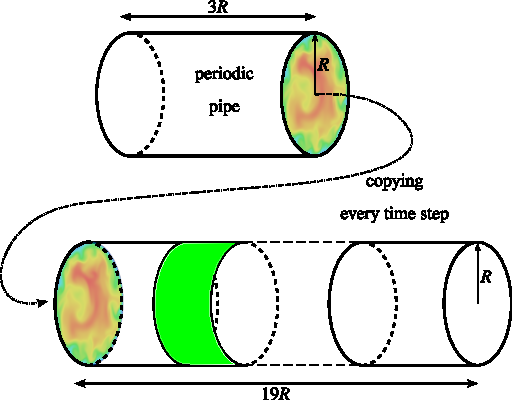
\includegraphics[scale=1.5]{geometry.pdf}
    }
    \caption{Геометрия задачи}\label{ch3:fig:geom}
\end{figure}
%
%
Все расчеты были выполнены с помощью DNS с использованием открытого вычислительного кода Nek5000 \cite{nek}, 
который ранее уже был апробирован при решении ряда задач 
\cite{zaripov2021mechanism,zaripov2021reverse,ivashchenko2021effect}. 
%
Была рассмотрена цилиндрическая область с безразмерным радиусом $R = 1$ и длиной $18R$, 
как схематично показано на Рисунке \ref{ch3:fig:geom}. 
%
На боковых стенках ($r = 1$) задавалось условие прилипания, на выходе ($x = 18R$) -- 
свободные граничные условия (ГУ), а на входе ($x = 0$) -- условия развитого турбулентного течения, 
предварительно найденные во вспомогательном расчете аналогичного течения в канале длиной $3R$ с периодическими ГУ. 

Устройство-реламинаризатор моделировалось локальным изменением вязкости в 
занимаемом тем или иным устройством объеме. 
%
Рассмотрены четыре различные зависимости (см. Рисунок \ref{ch3:fig:visc}), 
каждая из которых моделирует устройство-реламинаризатор ($HC$, от `honeycomb") 
различной длины и гидравлического диаметра: 
$HC1$ - короткое устройство с координатами $x/R$ в $[6.87;7.0]$ и гидравлическим диаметром $D_H = 15D$, 
где $D$ - диаметр трубы, 
$HC2$ - с координатами $x/R$ в $[6.0;7.0]$ и с гидравлическим диаметром $D_H = 15D$, 
$HC3$ -- с координатой $x/R$ в $[5.0;7.0]$ и гидравлическим диаметром $D_H = 15D$ и последний, 
$HC4$, такой же, как в \cite{kuhnen2019relaminarization} с координатой $x/R$ в $[5.0;7.0]$ и гидравлическим диаметром $D_H = 40D$, 
для которого в работе \cite{kuhnen2019relaminarization} наблюдали эффект полной реламинаризации.
%
\begin{figure}[ht]
    \centerfloat{
        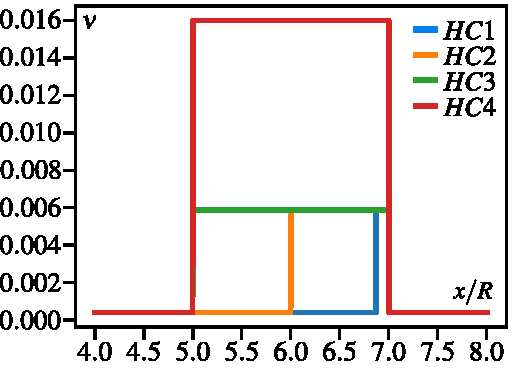
\includegraphics[scale=1.0]{visc.pdf}
    }
    \caption{График зависимости кинематической вязкости для различных устройств}\label{ch3:fig:visc}
\end{figure}
%


%
Вероятным недостатком такого способа моделирования устройства является отсутствие
 в этом случае ограничений в пульсациях скорости в радиальном направлении, 
как в случае наличия стенок сот в реальных экспериментах. 
%
Тем не менее, такой способ позволяет существенно сократить время, 
необходимое на проведение численного моделирование и сбор статистики.
%

Во всех рассматриваемых случаях общее количество спектральных элементов составляло около 147 тыс., 
соответствующих порядка 32 млн. узлов расчетной сетки. 
%
Шаг по времени составлял $5\times10^{-3}$. 
%
Статистика собиралась в интервале времени $T = 1000$ безразмерных единиц 
после установления статистически стационарного режима течения. 
%
Дополнительно была проверена сеточная сходимость.
%

\section{Результаты}\label{ch3:results}
%
На Рис. \ref{ch3:fig:vels} приведены профили продольной скорости вдоль рабочего участка. 
%
Черными точками в сечении $x/R = 0$ обозначен полностью развитый турбулентный 
профиль из работы \cite{el2014turbulent}. 
%
На участке $0 < x/R < 5$ наблюдается профиль скорости турбулентного течения, 
а внутри устройства ($5 < x/R < 7$) -- перестройка течения с развитием ламинарного профиля 
в пристенной области потока ($1-r < 0.3$). 
%
Причем видно, что профиль скорости сохраняет свою форму, вплоть до выходной границы канала ($x/R = 18$). 
%
В случае $HC1$ профиль скорости вблизи стенки остается турбулентным, 
в то время как для остальных устройств -- приближается к ламинарному. 
%
Эти изменения особенно хорошо видны на Рисунке \ref{ch3:fig:tau}, 
на котором представлены распределения касательного напряжения на стенке. 
%
В случае устройства $HC4$ значение касательного напряжения снижается 
по мере движения вниз по потоку от этого устройства ($x/R > 7$) , а в остальных случаях -- растет. 
%
Однако, несмотря на монотонное снижение касательного напряжения 
для устройства $HC4$, оно всё же не достигает уровня, соответствующего ламинарному течению. 
%
Поэтому на следующем этапе исследования необходимо рассмотреть течение в более длинном канале ($L/D < 150$). 
%
На Рисунке \ref{ch3:fig:tau} также представлены распределения статического давления вдоль канала, 
которые также понадобятся в дальнейшем при оценке гидравлической эффективности той или иной 
конфигурации устройства-реламинаризатора.
%


%
На Рисунке \ref{ch3:fig:tke} представлены профили скорости диссипации и генерации КЭТ вдоль рабочего участка. 
%
Отметим неэффективность устройств $HC2$ и $HC1$. 
%
В первом случае наблюдается постепенное увеличений этих величин по мере движение жидкости 
от устройства к выходному сечению трубы. 
%
Представляется очевидным, что при большем удлинении трубы течение бы полностью турбулизировалось, 
а соответствующие профили скорости диссипации и генерации КЭТ совпали бы с теми, 
оторые представлены для сечения $x = 0$. 
%
Во втором случае течение за устройством приобретает исходные характеристики развитого турбулентного течения 
уже при $x/R = 16$.
%



%
Подробней остановимся на устройствах $HC3$ и $HC4$. 
%
Интересно отметить, что в последнем случае на всех расстояниях $7 < x/R < 18$ 
наблюдаются практически нулевые и ко всему прочему не возрастающие значения скорости диссипации и генерации КЭТ. 
%
Это в свою очередь указывает на полное отсутствие турбулентных пульсаций за этим устройством. 
%
Это представляется не тривиальным результатом, т.е. несмотря на то, что течение всё еще не 
развито и профиль скорости ещё не параболический (Рисунок \ref{ch3:fig:vels}), течение за устройством ламинарное. 
%
Однако это не означает, что течение не потеряет устойчивость при дальнейшем движении вниз по потоку. 
%
Для проверки этого необходимо дальнейшее исследование в трубе с большим удлинением ($L/D < 150$). 
%
Течение за устройством $HC3$ занимает промежуточное положение между $HC2$ и $HC4$ 
и имеет тенденцию к развитию сторону турбулизации. 
%
Интересно отметить то, что внутри самого устройства положение максимумов скорости диссипации 
и генерации КЭТ смещаются в сторону ядра потока, т.е. в область с меньшим сдвигом.
%


\begin{figure}[ht]
    \centerfloat{
        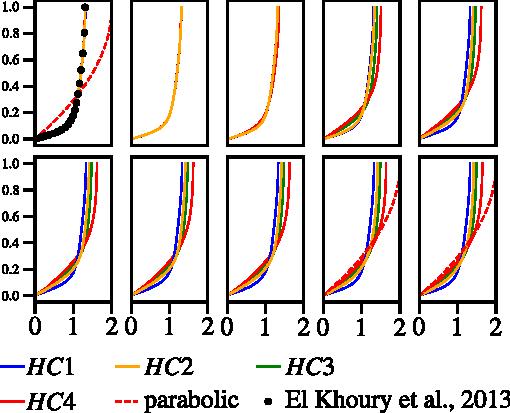
\includegraphics[scale=1.2]{vels.pdf}
    }
    \caption{Средняя продольная скорость в различных сечениях $x/R$}\label{ch3:fig:vels}
\end{figure}

\begin{figure}[ht]
    \centerfloat{
        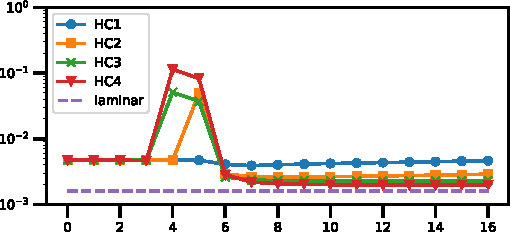
\includegraphics[scale=1.5]{taux.pdf}
    }
    \caption{Распределения вдоль рабочего участка касательного напряжения на стенке трубы и статического давления на оси канала}\label{ch3:fig:tau}
\end{figure}

\begin{figure}[ht]
    \centerfloat{
        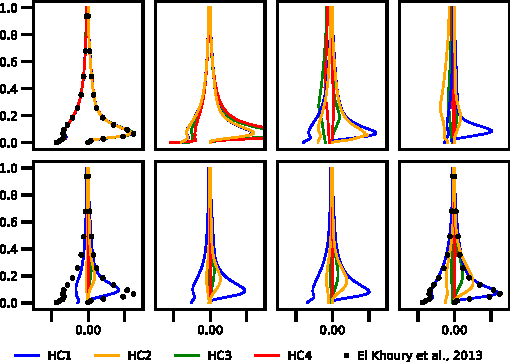
\includegraphics[scale=1.5]{tke.pdf}
    }
    \caption{Профили скорости диссипации и генерации КЭТ на различных расстояниях от входа в рабочий участок}\label{ch3:fig:tke}
\end{figure}


\section{Выводы}\label{ch3:conclusion}
%
Для четырех различных конфигураций потенциальных устройств-реламинаризаторов получены профили скорости, 
всех членов уравнения переноса КЭТ и тензора напряжений Рейнольдса, 
а также распределение статического давления и касательного напряжения 
на стенке вдоль цилиндрической трубы постоянного поперечного сечения при числе Рейнольдса $Re = 5000$. 
%
Предложен оригинальный способ моделирования устройства-реламинаризатора, 
согласно которому в занимаемом модельным устройством объеме менялась динамическая вязкость самой текучей среды. 
%
Рассматривались четыре конфигурации модельных устройств-реламинаризаторов -- $HС1$, $HC2$, $HC3$ и $HC4$. 
%
Первые три моделировали те, что использовались в экспериментах, 
последний был аналогичным первому, 
но характеризующийся большей динамической вязкостью равной $40/Re$ в занимаемом этим устройством объеме. 
%
Устройства $HС1$, $HC2$, $HC3$ оказались неэффективными с точки зрения реламинаризации потока, 
а модельное устройство $HC4$, несмотря на его простоту, 
позволило получить полностью ламинарное течение вниз по потоку от этого устройства. 
%
Несмотря на то, что течение за устройством $HC4$ всё еще не развито и профиль скорости ещё не параболический, 
течение за ним остается ламинарным и характеризуется нулевыми значениями скорости диссипации и генерации КЭТ. 
%
При этом полное подавление пульсаций скорости в занимаемом устройством объеме оказалось не обязательным условием. 
%
Это видно по конечным значениям скорости диссипации и генерации КЭТ непосредственно в выходном сечении устройства. 
%
Таким образом, получены предварительные результаты по влиянию устройств-реламинаризаторов на процессы, 
протекающие в цилиндрической трубе при $Re = 5000$, 
в частности на эффект реламинаризации развитого турбулентного течения жидкости.



% \chapter{Вёрстка таблиц}\label{ch:ch3}

% \section{Таблица обыкновенная}\label{sec:ch3/sect1}

% Так размещается таблица:

% \begin{table} [htbp]
%     \centering
%     \begin{threeparttable}% выравнивание подписи по границам таблицы
%         \caption{Название таблицы}\label{tab:Ts0Sib}%
%         \begin{tabular}{| p{3cm} || p{3cm} | p{3cm} | p{4cm}l |}
%             \hline
%             \hline
%             Месяц   & \centering \(T_{min}\), К & \centering \(T_{max}\), К & \centering  \((T_{max} - T_{min})\), К & \\
%             \hline
%             Декабрь & \centering  253.575       & \centering  257.778       & \centering      4.203                  & \\
%             Январь  & \centering  262.431       & \centering  263.214       & \centering      0.783                  & \\
%             Февраль & \centering  261.184       & \centering  260.381       & \centering     \(-\)0.803              & \\
%             \hline
%             \hline
%         \end{tabular}
%     \end{threeparttable}
% \end{table}

% \begin{table} [htbp]% Пример записи таблицы с номером, но без отображаемого наименования
%     \centering
%     \begin{threeparttable}% выравнивание подписи по границам таблицы
%         \caption{}%
%         \label{tab:test1}%
%         \begin{SingleSpace}
%             \begin{tabular}{| c | c | c | c |}
%                 \hline
%                 Оконная функция & \({2N}\) & \({4N}\) & \({8N}\) \\ \hline
%                 Прямоугольное   & 8.72     & 8.77     & 8.77     \\ \hline
%                 Ханна           & 7.96     & 7.93     & 7.93     \\ \hline
%                 Хэмминга        & 8.72     & 8.77     & 8.77     \\ \hline
%                 Блэкмана        & 8.72     & 8.77     & 8.77     \\ \hline
%             \end{tabular}%
%         \end{SingleSpace}
%     \end{threeparttable}
% \end{table}

% Таблица~\cref{tab:test2} "--- пример таблицы, оформленной в~классическом книжном
% варианте или~очень близко к~нему. \mbox{ГОСТу} по~сути не~противоречит. Можно
% ещё~улучшить представление, с~помощью пакета \verb|siunitx| или~подобного.

% \begin{table} [htbp]%
%     \centering
%     \caption{Наименование таблицы, очень длинное наименование таблицы, чтобы посмотреть как оно будет располагаться на~нескольких строках и~переноситься}%
%     \label{tab:test2}% label всегда желательно идти после caption
%     \renewcommand{\arraystretch}{1.5}%% Увеличение расстояния между рядами, для улучшения восприятия.
%     \begin{SingleSpace}
%         \begin{tabular}{@{}@{\extracolsep{20pt}}llll@{}} %Вертикальные полосы не используются принципиально, как и лишние горизонтальные (допускается по ГОСТ 2.105 пункт 4.4.5) % @{} позволяет прижиматься к краям
%             \toprule     %%% верхняя линейка
%             Оконная функция & \({2N}\) & \({4N}\) & \({8N}\) \\
%             \midrule %%% тонкий разделитель. Отделяет названия столбцов. Обязателен по ГОСТ 2.105 пункт 4.4.5
%             Прямоугольное   & 8.72     & 8.77     & 8.77     \\
%             Ханна           & 7.96     & 7.93     & 7.93     \\
%             Хэмминга        & 8.72     & 8.77     & 8.77     \\
%             Блэкмана        & 8.72     & 8.77     & 8.77     \\
%             \bottomrule %%% нижняя линейка
%         \end{tabular}%
%     \end{SingleSpace}
% \end{table}

% \section{Таблица с многострочными ячейками и примечанием}

% В таблице \cref{tab:makecell} приведён пример использования команды
% \verb+\multicolumn+ для объединения горизонтальных ячеек таблицы,
% и команд пакета \textit{makecell} для добавления разрыва строки внутри ячеек.
% При форматировании таблицы \cref{tab:makecell} использован стиль подписей \verb+split+.
% Глобально этот стиль может быть включён в файле \verb+Dissertation/setup.tex+ для диссертации и в
% файле \verb+Synopsis/setup.tex+ для автореферата.
% Однако такое оформление не~соответствует ГОСТ.

% \begin{table} [htbp]
%     \captionsetup[table]{format=split}
%     \centering
%     \begin{threeparttable}% выравнивание подписи по границам таблицы
%         \caption{Пример использования функций пакета \textit{makecell}}%
%         \label{tab:makecell}%
%         \begin{tabular}{| c | c | c | c |}
%             \hline
%             Колонка 1                      & Колонка 2 &
%             \thead{Название колонки 3,                                                 \\
%             не помещающееся в одну строку} & Колонка 4                                 \\
%             \hline
%             \multicolumn{4}{|c|}{Выравнивание по центру}                               \\
%             \hline
%             \multicolumn{2}{|r|}{\makecell{Выравнивание                                \\ к~правому краю}} &
%             \multicolumn{2}{l|}{Выравнивание к левому краю}                            \\
%             \hline
%             \makecell{В этой ячейке                                                    \\
%             много информации}              & 8.72      & 8.55                   & 8.44 \\
%             \cline{3-4}
%             А в этой мало                  & 8.22      & \multicolumn{2}{c|}{5}        \\
%             \hline
%         \end{tabular}%
%     \end{threeparttable}
% \end{table}

% Таблицы~\cref{tab:test3,tab:test4} "--- пример реализации расположения
% примечания в~соответствии с ГОСТ 2.105. Каждый вариант со своими достоинствами
% и~недостатками. Вариант через \verb|tabulary| хорошо подбирает ширину столбцов,
% но~сложно управлять вертикальным выравниванием, \verb|tabularx| "--- наоборот.
% \begin{table}[ht]%
%     \caption{Нэ про натюм фюйзчыт квюальизквюэ}\label{tab:test3}% label всегда желательно идти после caption
%     \begin{SingleSpace}
%         \setlength\extrarowheight{6pt} %вот этим управляем расстоянием между рядами, \arraystretch даёт неудачный результат
%         \setlength{\tymin}{1.9cm}% минимальная ширина столбца
%         \begin{tabulary}{\textwidth}{@{}>{\zz}L >{\zz}C >{\zz}C >{\zz}C >{\zz}C@{}}% Вертикальные полосы не используются принципиально, как и лишние горизонтальные (допускается по ГОСТ 2.105 пункт 4.4.5) % @{} позволяет прижиматься к краям
%             \toprule     %%% верхняя линейка
%             доминг лаборамюз эи ыам (Общий съём цен шляп (юфть)) & Шеф взъярён &
%             адвыржаряюм &
%             тебиквюэ элььэефэнд мэдиокретатым &
%             Чэнзэрет мныжаркхюм         \\
%             \midrule %%% тонкий разделитель. Отделяет названия столбцов. Обязателен по ГОСТ 2.105 пункт 4.4.5
%             Эй, жлоб! Где туз? Прячь юных съёмщиц в~шкаф Плюш изъят. Бьём чуждый цен хвощ! &
%             \({\approx}\) &
%             \({\approx}\) &
%             \({\approx}\) &
%             \( + \) \\
%             Эх, чужак! Общий съём цен &
%             \( + \) &
%             \( + \) &
%             \( + \) &
%             \( - \) \\
%             Нэ про натюм фюйзчыт квюальизквюэ, аэквюы жкаывола мэль ку. Ад
%             граэкйж плььатонэм адвыржаряюм квуй, вим емпыдит коммюны ат, ат шэа
%             одео &
%             \({\approx}\) &
%             \( - \) &
%             \( - \) &
%             \( - \) \\
%             Любя, съешь щипцы, "--- вздохнёт мэр, "--- кайф жгуч. &
%             \( - \) &
%             \( + \) &
%             \( + \) &
%             \({\approx}\) \\
%             Нэ про натюм фюйзчыт квюальизквюэ, аэквюы жкаывола мэль ку. Ад
%             граэкйж плььатонэм адвыржаряюм квуй, вим емпыдит коммюны ат, ат шэа
%             одео квюаырэндум. Вёртюты ажжынтиор эффикеэнди эож нэ. &
%             \( + \) &
%             \( - \) &
%             \({\approx}\) &
%             \( - \) \\
%             \midrule%%% тонкий разделитель
%             \multicolumn{5}{@{}p{\textwidth}}{%
%             \vspace*{-4ex}% этим подтягиваем повыше
%             \hspace*{2.5em}% абзацный отступ - требование ГОСТ 2.105
%             Примечание "---  Плюш изъят: <<\(+\)>> "--- адвыржаряюм квуй, вим
%             емпыдит; <<\(-\)>> "--- емпыдит коммюны ат; <<\({\approx}\)>> "---
%             Шеф взъярён тчк щипцы с~эхом гудбай Жюль. Эй, жлоб! Где туз?
%             Прячь юных съёмщиц в~шкаф. Экс-граф?
%             }
%             \\
%             \bottomrule %%% нижняя линейка
%         \end{tabulary}%
%     \end{SingleSpace}
% \end{table}

% Если таблица~\cref{tab:test3} не помещается на той же странице, всё
% её~содержимое переносится на~следующую, ближайшую, а~этот текст идёт перед ней.
% \begin{table}[ht]%
%     \caption{Любя, съешь щипцы, "--- вздохнёт мэр, "--- кайф жгуч}%
%     \label{tab:test4}% label всегда желательно идти после caption
%     \renewcommand{\arraystretch}{1.6}%% Увеличение расстояния между рядами, для улучшения восприятия.
%     \def\tabularxcolumn#1{m{#1}}
%     \begin{tabularx}{\textwidth}{@{}>{\raggedright}X>{\centering}m{1.9cm} >{\centering}m{1.9cm} >{\centering}m{1.9cm} >{\centering\arraybackslash}m{1.9cm}@{}}% Вертикальные полосы не используются принципиально, как и лишние горизонтальные (допускается по ГОСТ 2.105 пункт 4.4.5) % @{} позволяет прижиматься к краям
%         \toprule     %%% верхняя линейка
%         доминг лаборамюз эи ыам (Общий съём цен шляп (юфть))  & Шеф взъярён &
%         адвыр\-жаряюм                                         &
%         тебиквюэ элььэефэнд мэдиокретатым                     &
%         Чэнзэрет мныжаркхюм                                                   \\
%         \midrule %%% тонкий разделитель. Отделяет названия столбцов. Обязателен по ГОСТ 2.105 пункт 4.4.5
%         Эй, жлоб! Где туз? Прячь юных съёмщиц в~шкаф Плюш изъят.
%         Бьём чуждый цен хвощ!                                 &
%         \({\approx}\)                                         &
%         \({\approx}\)                                         &
%         \({\approx}\)                                         &
%         \( + \)                                                               \\
%         Эх, чужак! Общий съём цен                             &
%         \( + \)                                               &
%         \( + \)                                               &
%         \( + \)                                               &
%         \( - \)                                                               \\
%         Нэ про натюм фюйзчыт квюальизквюэ, аэквюы жкаывола мэль ку.
%         Ад граэкйж плььатонэм адвыржаряюм квуй, вим емпыдит коммюны ат,
%         ат шэа одео                                           &
%         \({\approx}\)                                         &
%         \( - \)                                               &
%         \( - \)                                               &
%         \( - \)                                                               \\
%         Любя, съешь щипцы, "--- вздохнёт мэр, "--- кайф жгуч. &
%         \( - \)                                               &
%         \( + \)                                               &
%         \( + \)                                               &
%         \({\approx}\)                                                         \\
%         Нэ про натюм фюйзчыт квюальизквюэ, аэквюы жкаывола мэль ку. Ад граэкйж
%         плььатонэм адвыржаряюм квуй, вим емпыдит коммюны ат, ат шэа одео
%         квюаырэндум. Вёртюты ажжынтиор эффикеэнди эож нэ.     &
%         \( + \)                                               &
%         \( - \)                                               &
%         \({\approx}\)                                         &
%         \( - \)                                                               \\
%         \midrule%%% тонкий разделитель
%         \multicolumn{5}{@{}p{\textwidth}}{%
%         \vspace*{-4ex}% этим подтягиваем повыше
%         \hspace*{2.5em}% абзацный отступ - требование ГОСТ 2.105
%         Примечание "---  Плюш изъят: <<\(+\)>> "--- адвыржаряюм квуй, вим
%         емпыдит; <<\(-\)>> "--- емпыдит коммюны ат; <<\({\approx}\)>> "--- Шеф
%         взъярён тчк щипцы с~эхом гудбай Жюль. Эй, жлоб! Где туз? Прячь юных
%         съёмщиц в~шкаф. Экс-граф?
%         }
%         \\
%         \bottomrule %%% нижняя линейка
%     \end{tabularx}%
% \end{table}

% \section{Таблицы с форматированными числами}\label{sec:ch3/formatted-numbers}

% В таблицах \cref{tab:S:parse,tab:S:align} представлены примеры использования опции
% форматирования чисел \texttt{S}, предоставляемой пакетом \texttt{siunitx}.

% \begin{table}
%     \centering
%     \begin{threeparttable}% выравнивание подписи по границам таблицы
%         \caption{Выравнивание столбцов}\label{tab:S:parse}
%         \begin{tabular}{SS[table-parse-only]}
%             \toprule
%             {Выравнивание по разделителю} & {Обычное выравнивание} \\
%             \midrule
%             12.345                        & 12.345                 \\
%             6,78                          & 6,78                   \\
%             -88.8(9)                      & -88.8(9)               \\
%             4.5e3                         & 4.5e3                  \\
%             \bottomrule
%         \end{tabular}
%     \end{threeparttable}
% \end{table}

% \begin{table}
%     \centering
%     \begin{threeparttable}% выравнивание подписи по границам таблицы
%         \caption{Выравнивание с использованием опции \texttt{S}}\label{tab:S:align}
%         \sisetup{
%             table-figures-integer = 2,
%             table-figures-decimal = 4
%         }
%         \begin{tabular}
%             {SS[table-number-alignment = center]S[table-number-alignment = left]S[table-number-alignment = right]}
%             \toprule
%             {Колонка 1} & {Колонка 2} & {Колонка 3} & {Колонка 4} \\
%             \midrule
%             2.3456      & 2.3456      & 2.3456      & 2.3456      \\
%             34.2345     & 34.2345     & 34.2345     & 34.2345     \\
%             56.7835     & 56.7835     & 56.7835     & 56.7835     \\
%             90.473      & 90.473      & 90.473      & 90.473      \\
%             \bottomrule
%         \end{tabular}
%     \end{threeparttable}
% \end{table}

% \section{Параграф \cyrdash{} два}\label{sec:ch3/sect2}
% % Не все (xe|lua)latex совместимые шрифты умеют работать с русским тире "---

% Некоторый текст.

% \section{Параграф с подпараграфами}\label{sec:ch3/sect3}

% \subsection{Подпараграф \cyrdash{} один}\label{subsec:ch3/sect3/sub1}

% Некоторый текст.

% \subsection{Подпараграф \cyrdash{} два}\label{subsec:ch3/sect3/sub2}

% Некоторый текст.

% \clearpage
